\section{Flächenträgheitsmomente}
    \begin{center}
    \vspace{-2mm}
        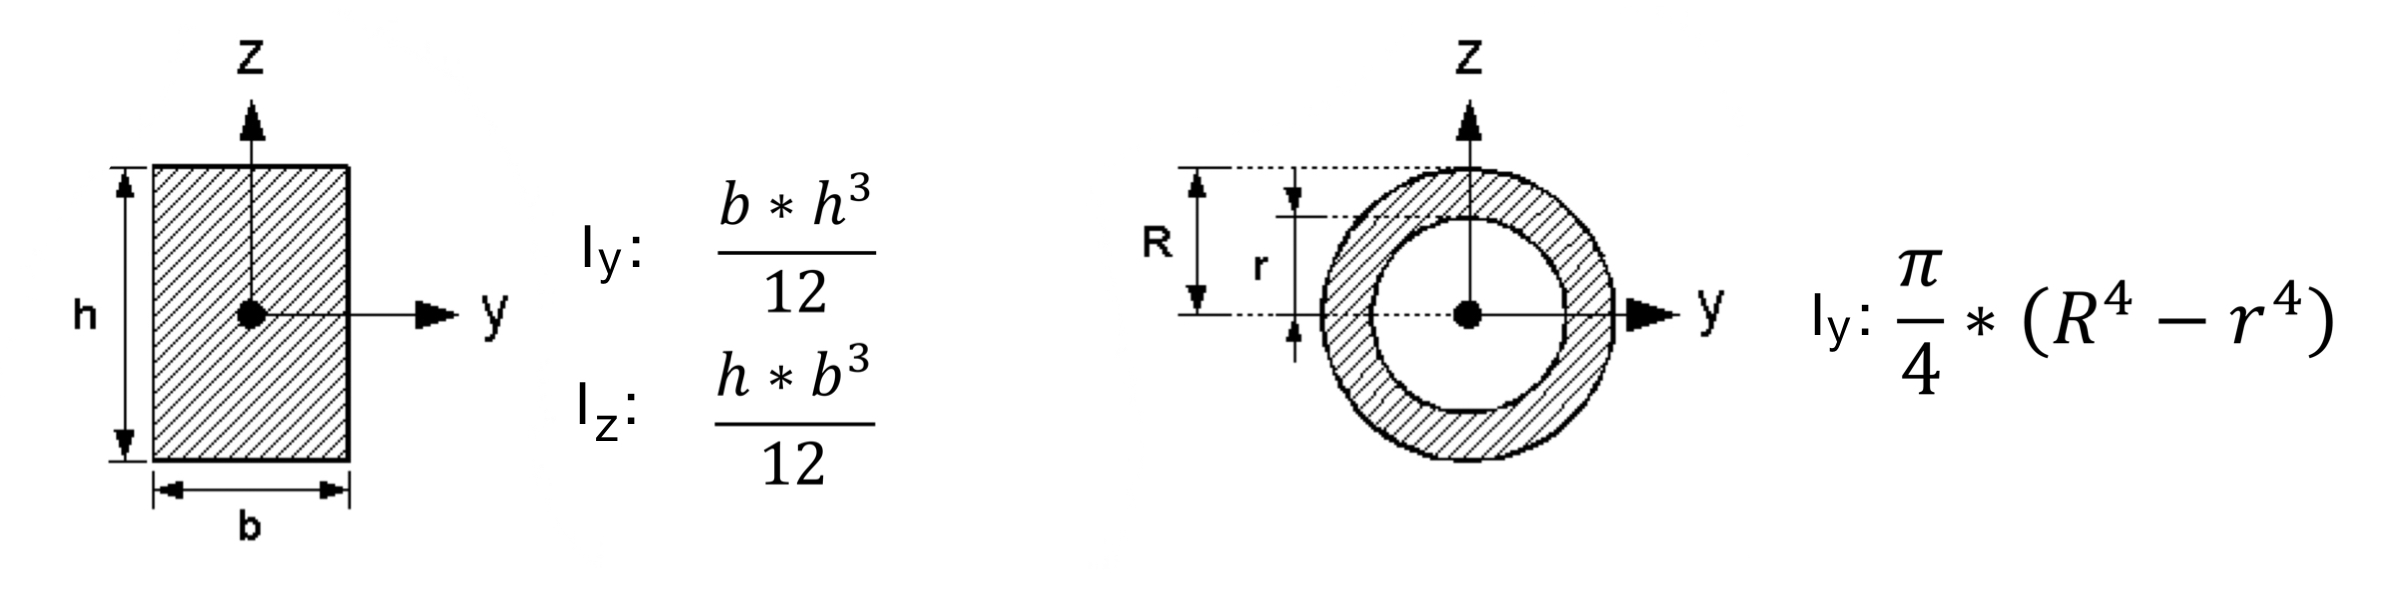
\includegraphics[width= 0.8\linewidth,]{10/traegheitsmom.jpeg}
    \end{center}
%\vspace{-3mm}
\section{Kesselgleichungen}
    %\vspace{1mm}
    Für \textbf{geschlossene}, dünnwandige Behälter ($\frac{d}{R} \ll 1$):
    %\vspace{-2mm}
    \[\sigma_{\varphi\varphi} = \frac{R}{d}P = 2\sigma_{zz}; \quad \sigma_{zz} = \frac{R}{2d}P \textrm{ }(\textrm{offen: }\sigma_{zz}=0); \quad \sigma_{rr}=0\]
    Für dünnwandige, \textbf{kugelförmige} Behälter:
    %\vspace{-2mm}
    \[\sigma_{\varphi\varphi}=\sigma_{\theta\theta}=\frac{R}{2d}P; \quad \sigma_{rr}=0\]


% \section{Relationen}
%     \vspace{1mm}
%     \[\textrm{Biegung: }\sigma_{xx}=-\frac{M_{z}(x)}{I}\cdot y, \quad\textrm{Normalkraft: }\sigma_{xx}=\frac{N(x)}{A}\]
%     \vspace{1mm}